\graphicspath{{./figures/}}
\title{compilation steps / C}
\date{}
\usepackage{cancel}
\begin{document}
\begin{frame}
    \titlepage
\end{frame}
\newmintinline{c}{}
\newminted{c}{linenos=true,xleftmargin=1cm,beameroverlays,escapeinside=@@,texcomments}
\newminted[ccodeNL]{c}{linenos=false,beameroverlays,escapeinside=@@,texcomments}
\newminted[ccodeS]{c}{linenos=false,fontsize=\small,beameroverlays,escapeinside=@@,texcomments}
\lstnewenvironment{asmcodeNL}{\lstset{language=myasm,escapeinside=@@,deletekeywords=test,texcl=false}}{}
\lstnewenvironment{asmcodeS}{\lstset{language=myasm,style=small,escapeinside=@@}}{}
\lstnewenvironment{asmcodeT}{\lstset{language=myasm,style=smaller,escapeinside=@@}}{}

\input{../common/highBoxLib}
\tikzset{
    program memory label/.style={font=\ttfamily},
    program memory box/.style={draw,rectangle,minimum width=5cm,fill=white},
    program memory highlight/.style={draw,rectangle,line width=1mm, draw=blue!80!black,opacity=.3,
        inner sep=0.5mm},
}

\newcommand{\programMemoryImage}{
\node[program memory box,minimum height=1cm,pattern=north west lines,pattern color=black!5!white] (kernel) {Used by OS};
\node[right=1mm of kernel.north east,program memory label] {0xFFFF FFFF FFFF FFFF};
\node[right=1mm of kernel.south east,program memory label] {0xFFFF 8000 0000 0000};
\node[program memory box, minimum height=.5cm, below=1cm of kernel] (stack) {Stack};
\node[right=1mm of stack.north east,program memory label] {0x7F\ldots{}};
\node[program memory box, minimum height=.5cm, below=1cm of stack] (heap) {Heap / other dynamic};
\node[program memory box, minimum height=.5cm, below=0mm of heap] (data) {Writable data};
\node[program memory box, minimum height=.5cm, below=0mm of data] (sdata) {Code + Constants};
\node[right=1mm of sdata.south east,program memory label] {0x0000 0000 0040 0000};
\coordinate (memBottom) at ($(sdata.south east) + (0mm, -2mm)$);
\begin{pgfonlayer}{bg}
\draw[pattern=north west lines, pattern color=black!40!white] (kernel.north west) rectangle (memBottom);
\end{pgfonlayer}
}
\newcommand{\programMemoryHighlight}[1]{
    \node[#1,program memory highlight] {};
}




\section{Compilation Steps}

\subsection{Intro: Program Layout}

% FIXME: consider moving?
\usetikzlibrary{calc,decorations.pathreplacing,fit,matrix,patterns,positioning}

\begin{frame}{program memory (x86-64 Linux)}
\begin{tikzpicture}
\programMemoryImage
\begin{visibleenv}<2-3>
\programMemoryHighlight{fit=(stack)}
    \foreach \x in {-1cm,0cm,1cm} {
        \draw[-latex,line width=1mm,red!80!black,xshift=\x] (stack.south) ++ (\x,0cm) -- +(0cm, -.5cm);
    };
\end{visibleenv}
\begin{visibleenv}<2|handout:1>
    \node[below right=1mm of stack.south east,align=left,fill=blue!10!white] {stack \myemph{grows down} \\ ``top'' has smallest address};
\end{visibleenv}
\begin{pgfonlayer}{fg}
\begin{visibleenv}<3|handout:2>
    \matrix (stackFrame) [matrix of nodes,
        row sep=0mm,
        inner sep=0mm,
        font=\small,
        nodes={draw,rectangle,minimum width=4cm,minimum height=4mm,fill=white,align=center},
        right=15mm of stack.south east,
        fill=white,opacity=0.9,
        outer sep=4mm
    ] {
        \ldots \\
        argument 6 \\
        argument 7 \\
        \ldots \\
        return address \\
        |[minimum height=1cm]| callee saved registers \\
        |[minimum height=.5cm]| local variables \\
        |[]| {\textit{(next thing on stack)}} \\
    };
\end{visibleenv}
\end{pgfonlayer}
\begin{visibleenv}<4|handout:0>
    \programMemoryHighlight{fit=(stack.south west) (heap.north east)}
    \programMemoryHighlight{fit=(kernel.north west) (stack.north east)}
    \programMemoryHighlight{fit=(sdata.south west) (memBottom)}
\end{visibleenv}
\begin{visibleenv}<5|handout:0>
    \draw[ultra thick,decorate,decoration=brace] ([xshift=1mm]data.north east) -- ([xshift=1mm]sdata.south east) node[midway,right] {
        loaded from executable file
    };
    \programMemoryHighlight{fit=(sdata.south west) (data.north east)}
\end{visibleenv}
\end{tikzpicture}
\end{frame}


\subsection{Compilation Pipeline}

\usetikzlibrary{arrows.meta,calc,chains,fit}

\begin{frame}[fragile,label=compilation]{compilation pipeline}
\begin{tikzpicture}
\begin{scope}[start chain=going below, every node/.style={on chain,join,font=\small},every join/.style={-Latex,thick},node distance=1cm]
\node[draw,align=center] (mainC) {main.c \\ (C code)};
\node {compile};
\node[draw,align=center] {main.s \\ (assembly)};
\node {assemble};
\node[draw,align=center,on chain=going right] {main.o \\ (object file) \\ (machine code)};
\node[on chain=going right] (linking) {linking};
\node[draw,align=center,on chain=going right] {main.exe \\ (executable) \\ (machine code)};
\end{scope}
\begin{visibleenv}<2->
\node[align=left,font=\small,anchor=north west] at ([xshift=1cm]mainC.north east){
main.c: \\
\begin{minipage}{\textwidth}
\begin{minted}{c}
#include <stdio.h>
int main(void) {
    printf("Hello, World!\n");
}
\end{minted}
\end{minipage}
};
\end{visibleenv}
\begin{visibleenv}<3->
\node[above=.5cm of linking,draw,align=center,red!90!black,font=\small] (printfO) { printf.o \\ (object file) };
\draw[red,-Latex,thick] (printfO) -- (linking.north);
\end{visibleenv}
\end{tikzpicture}
\end{frame}

\begin{frame}{compilation commands}
\begin{tabular}{llll}
\myemph{compile}: &\texttt{gcc -S file.c} & $\Rightarrow$ & \texttt{file.s} (assembly)\\
    \myemph{assemble}: & \texttt{gcc -c file.s} & $\Rightarrow$ &\texttt{file.o} (object file)\\
\myemph{link}: & \texttt{gcc -o file file.o} & $\Rightarrow$ & \texttt{file} (executable) \\
~&~&~\\
c+a: &\texttt{gcc -c file.c} & $\Rightarrow$ & \texttt{file.o} \\
c+a+l: &\texttt{gcc -o file file.c} & $\Rightarrow$ & \texttt{file} \\
\ldots{} & & & \\
\end{tabular}
\end{frame}

    % FIXME: diagram of memory layout with parts of object files?

\subsection{What's in those files?}

\usetikzlibrary{arrows.meta,calc,chains,fit}

\begin{frame}[label=compPipe,fragile]{what's in those files?}
\newcommand{\firstC}{1}
\newcommand{\firstS}{2}
\newcommand{\intelS}{3}
\newcommand{\markSub}{4}
\newcommand{\markXor}{5}
\newcommand{\firstOCode}{6}
\newcommand{\firstOData}{7}
\newcommand{\firstSOCorrespond}{8}
\newcommand{\firstOReloc}{9}
\newcommand{\firstOSymbols}{10}
\newcommand{\firstExe}{11}
    \lstset{
        language=[x8664gas]Assembler,
        %moredelim=**[is][\color{green!60!black}]{@1*}{*@},
        moredelim=**[is][\cbA<\firstSOCorrespond->]{@1*}{*@},
        moredelim=**[is][\cbB<\firstSOCorrespond->]{@2*}{*@},
        moredelim=**[is][\cbC<\firstSOCorrespond->]{@3*}{*@},
        moredelim=**[is][\cbD<\firstSOCorrespond->]{@4*}{*@},
        moredelim=**[is][\cbE<\markXor>]{@X*}{*@},
        moredelim=**[is][\cbF<\markSub>]{@S*}{*@},
        escapechar=`,
    }
    \vspace{-.5cm}
    \begin{tikzpicture}
    \tikzset{
        mybox part/.style={minimum width=2cm,font=\scriptsize,align=left},
        mybox/.style={draw,rectangle,mybox part},
        mybox thin/.style={draw,rectangle,mybox part,minimum width=1.5cm},
        mylabel/.style 2 args={label={[label distance=-1mm,inner sep=1mm,fill=white,draw,rectangle,font=\footnotesize,visible on=#2]90:#1}},
        mylabel red/.style 2 args={label={[label distance=-1mm,inner sep=1mm,fill=white,draw=red!70!black,very thick,dotted,rectangle,font=\footnotesize,visible on=#2]90:#1}},
        myline/.style={line width=1pt,-latex},
    }
    \makeatletter
    \newenvironment{mycolorbox}[1]
    {\def\savedcolor{#1}\begin{lrbox}{\@tempboxa}\strut}
    {\end{lrbox}\setlength{\fboxsep}{0pt}\colorbox{\savedcolor}{\usebox{\@tempboxa}}}
    \makeatother
    \def\doEndEnv{\end{mycolorbox}\egroup}
    \newcommand<>{\cbA}{\only#1{\begin{mycolorbox}{blue!40!white}\bgroup\aftergroup\doEndEnv}}
    \newcommand<>{\cbB}{\only#1{\begin{mycolorbox}{green!30!white}\bgroup\aftergroup\doEndEnv}}
    \newcommand<>{\cbC}{\only#1{\begin{mycolorbox}{red!20!white}\bgroup\aftergroup\doEndEnv}}
    \newcommand<>{\cbD}{\only#1{\begin{mycolorbox}{orange!30!white}\bgroup\aftergroup\doEndEnv}}
    \newcommand<>{\cbE}{\only#1{\begin{mycolorbox}{violet!30!white}\bgroup\aftergroup\doEndEnv}}
    \newcommand<>{\cbF}{\only#1{\begin{mycolorbox}{magenta!40!white}\bgroup\aftergroup\doEndEnv}}

    \node[mybox,mylabel={hello.c}{<\firstC->}] (helloC){
        \begin{minipage}{4cm}
\begin{ccode*}{xleftmargin=0cm,linenos=false}
#include <stdio.h>
int main(void) {
  puts("Hello, World!");
  return 0;
}
\end{ccode*} 
        \end{minipage}
    };

    \node[mybox,mylabel={hello.s}{<\firstS->},anchor=north west,visible on=<\firstS->] (helloS) at ($(helloC.north east) + (2cm, 0)$) {
\begin{lstlisting}
    .text
main:
    @S*@2*sub  $8, %rsp*@*@
    mov  $@1*.Lstr*@, %rdi
    call @3*puts*@
    @X*xor  %eax, %eax*@
    @S*add  $8, %rsp*@
    ret

    .data
@1*.Lstr*@: .string @4*"Hello, World!"*@
\end{lstlisting} 
    };

\begin{visibleenv}<\intelS>
        \node[overlay,mybox thin,mylabel red={hello.s (Intel syntax)}{<\firstS->},anchor=west,visible on=<\firstS->,fill=white,draw=red!70!black,dotted,ultra thick] (helloSIntel) at ($(helloS.east) + (-1cm, .5cm)$) {
\begin{lstlisting}
.text
main: 
  sub RSP, 8
  mov RDI, .Lstr
  call puts
  xor EAX, EAX
  add RSP, 8
  ret

.data
.Lstr: .string "Hello, World!"
\end{lstlisting} 
};
\end{visibleenv}

    \begin{visibleenv}<\markXor>
        \draw[red,very thick,Latex-] ([yshift=-2cm,xshift=-2cm]helloS.north east) coordinate (xorEnd) -- ++(1.75cm,0cm)
            coordinate (xorLast);
        \node[align=left,font=\small,thick,draw=red,anchor=west,fill=white] at (xorLast) {
            sets eax to 0 \\
            (shorter machine \\
            code than mov)
        };
    \end{visibleenv}

    \begin{visibleenv}<\markSub>
        \draw[red,very thick,Latex-] ([yshift=-1cm,xshift=-2.25cm]helloS.north east) coordinate (subEnd) -- ++(2cm,0cm)
            coordinate (subLast);
        \draw[red,very thick,Latex-] ([yshift=-2.3cm,xshift=-2.25cm]helloS.north east) coordinate (addEnd) -- ++(2cm,0cm)
            coordinate (addLast);
        \node[align=left,font=\small,thick,draw=red,anchor=west,fill=white] at ($(subLast)!0.5!(addLast)$) {
            Linux x86-64 \\
            calling convention: \\
            stack addr. must be \\
            multiple of 16
        };
    \end{visibleenv}

    \draw[myline,visible on=<\firstS->] (helloC) -- (helloS);
    
    \node[mybox part,visible on=<\firstOCode->,anchor=north west,inner sep=.5mm] (helloOText) at ($(helloC.south west) + (0, -1cm)$) {
        \textbf{text} (code) segment: \\
        \texttt{{\cbB<\firstSOCorrespond->48 83 EC 08} BF {\cbA<\firstSOCorrespond->00 00 00 00} E8 {\cbC<\firstSOCorrespond->00 00}} \\
        \texttt{{\cbC<\firstSOCorrespond->00 00} 31 C0 48 83 C4 08 C3}
    };
    \node[mybox part,visible on=<\firstOData->,anchor=north west,inner sep=.5mm] (helloOData) at (helloOText.south west) {
        \textbf{data} segment: \\
        \texttt{{\cbD<\firstSOCorrespond->48 65 6C 6C 6F 2C 20 57 6F 72 6C 00}}
    };
    \node[mybox part,visible on=<\firstOReloc->,anchor=north west,inner sep=.5mm] (helloOReloc) at (helloOData.south west) {
        \textbf{relocations}: \\
        \begin{tabular}{ll}
        \it take 0s at & \it and replace with \\
        text, byte 5 ({\cbA$\;$}) & data segment, byte 0 \\
        text, byte 10 ({\cbC$\;$}) & address of \texttt{puts} \\
        \end{tabular}
    };
    \node[mybox part,visible on=<\firstOSymbols->,anchor=north west,inner sep=.5mm] (helloOSymbols) at (helloOReloc.south west) {
        \textbf{symbol table}: \\
        \begin{tabular}{ll}
        \tt main & text byte 0 \\
        \end{tabular} 
    };
    \node[mybox,mylabel={hello.o}{<\firstOCode->},anchor=north west,visible on=<\firstOCode->,
          fit=(helloOText) (helloOSymbols),inner sep=0mm] (helloO) {};

    \draw[myline,visible on=<\firstOCode->] (helloS) -- ($(helloO.north east) + (-1cm,0)$);

    \node[mybox,mylabel={hello.exe}{<\firstExe->},anchor=north west,visible on=<\firstExe->] (helloExe) at ($(helloS.south west) + (0, -1cm)$) {
        (actually binary, but shown as hexadecimal)
        \ldots \\
        \texttt{{\cbB 48 83 EC 08} BF {\cbA A7 02 04 00}} \\
        \texttt{E8 {\cbC 08 4A 00 00} 31 C0 48} \\
        \texttt{83 C4 08 C3} \ldots \\
        \ldots (code from stdio.o) \ldots \\
        \texttt{{\cbD 48 65 6C 6C 6F 2C 20 57 6F}} \\
        \texttt{{\cbD 72 6C 00}} \ldots \\
        \ldots (data from stdio.o) \ldots
    };

    \draw[myline,visible on=<\firstExe->] ($(helloO.east) + (0, 1cm)$) -- ($(helloExe.north) + (-1cm, 0)$) 
        node[midway,font=\footnotesize,rectangle,fill=white,draw,thin] {+ stdio.o};
    \end{tikzpicture}
\end{frame}

\begin{frame}[fragile,label=realHelloS]{hello.s}
\begin{Verbatim}
        .section        .rodata.str1.1,"aMS",@progbits,1
.LC0:
        .string "Hello, World!"
        .text
        .globl  main
main:
        subq    $8, %rsp
        movl    $.LC0, %edi
        call    puts
        movl    $0, %eax
        addq    $8, %rsp
        ret
\end{Verbatim}
\end{frame}


\subsection{Exercises}


\begin{frame}[fragile,label=exCL]{exercise (1)}
main.c: \\
\begin{ccode}
#include <stdio.h>
void sayHello(void) {
    puts("Hello, World!");
}
int main(void) {
    sayHello();
}
\end{ccode}
Which files contain the \textbf{memory address} of \texttt{sayHello}?
\begin{tabular}{ll}
\textit{A.} main.s (assembly) & \textit{D.} B and C \\
\textit{B.} main.o (object) &  \textit{E.} A, B and C \\
\textit{C.} main.exe (executable) & \textit{F.} something else \\
\end{tabular}
\end{frame}

\begin{frame}[fragile,label=exCL2]{exercise (2)}
main.c: \\
\begin{ccode}
#include <stdio.h>
void sayHello(void) {
    puts("Hello, World!");
}
int main(void) {
    sayHello();
}
\end{ccode}
Which files contain the \textbf{literal ASCII string} of \texttt{Hello, World!}?
\begin{tabular}{ll}
\textit{A.} main.s (assembly) & \textit{D.} B and C \\
\textit{B.} main.o (object) &  \textit{E.} A, B and C \\
\textit{C.} main.exe (executable) & \textit{F.} something else \\
\end{tabular}
\end{frame}
  % exercise 2

\subsection{aside: dynamic linking}
\begin{frame}{dynamic linking (very briefly)}
    \begin{itemize}
        \item \textit{dynamic linking} --- done \myemph{when application is loaded}
            \begin{itemize}
                \item idea: don't have $N$ copies of {\tt printf} on disk
                \item other type of linking: \textit{static} ({\tt gcc -static})
            \end{itemize}
        \item load executable file + its libraries into memory when app starts
        \item often extra indirection:
            \begin{itemize}
            \item {\tt call functionTable[number\_for\_printf]}
            \item linker fills in {\tt functionTable} instead of changing {\tt call}s
            \end{itemize}
    \end{itemize}
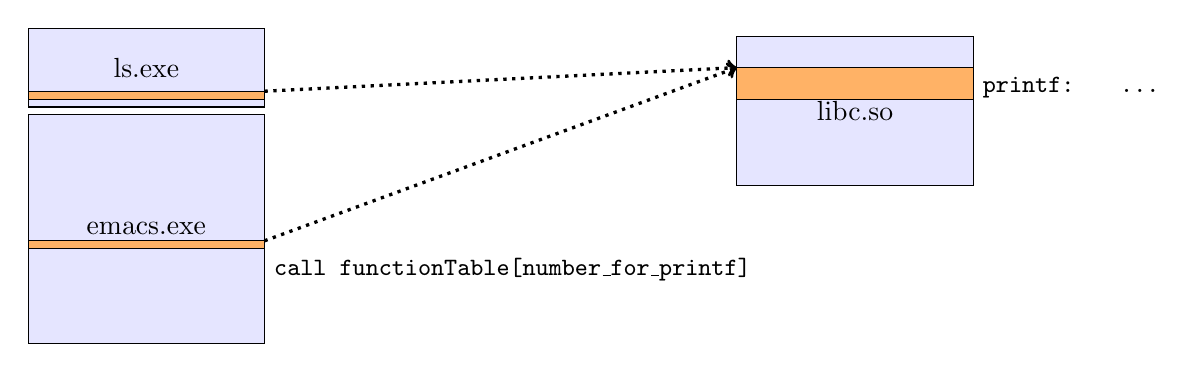
\begin{tikzpicture}
    \draw[fill=blue!10] (0, 0) rectangle (3, -1) node[midway] {ls.exe};
    \draw[fill=blue!10] (0, -1.1) rectangle (3, -4) node[midway] {emacs.exe};
    \draw[fill=blue!10] (9, -0.1) rectangle (12, -2) node[midway] {libc.so};
    \draw[fill=orange!60] (0, -.8) rectangle (3, -.9);
    \draw[fill=orange!60] (0, -2.7) rectangle (3, -2.8);
    \draw[fill=orange!60] (9, -0.5) rectangle (12, -0.9);
    \draw[very thick,->,dotted] (3, -.8) -- (9, -0.5);
    \draw[very thick,->,dotted] (3, -2.7) -- (9, -0.5);
    \node[anchor=north west,font=\fontsize{9}{10}\tt\selectfont] at (3, -2.8) {
        call functionTable[number\_for\_printf]
    };
    \node[anchor=north west,font=\fontsize{9}{10}\tt\selectfont] at (12, -0.5) {
        printf: \\
        \hspace{.25cm} \ldots
    };
\end{tikzpicture}
\end{frame}

\begin{frame}[fragile,label=lddBinLs]{\tt ldd /bin/ls}
\begin{Verbatim}[fontsize=\fontsize{12}{13}\selectfont]
$ ldd /bin/ls
    linux-vdso.so.1 =>  (0x00007ffcca9d8000)
    libselinux.so.1 => /lib/x86_64-linux-gnu/libselinux.so.1
            (0x00007f851756f000)
    libc.so.6 => /lib/x86_64-linux-gnu/libc.so.6
            (0x00007f85171a5000)
    libpcre.so.3 => /lib/x86_64-linux-gnu/libpcre.so.3
            (0x00007f8516f35000)
    libdl.so.2 => /lib/x86_64-linux-gnu/libdl.so.2
            (0x00007f8516d31000)
    /lib64/ld-linux-x86-64.so.2 (0x00007f8517791000)
    libpthread.so.0 => /lib/x86_64-linux-gnu/libpthread.so.0
            (0x00007f8516b14000)
\end{Verbatim}
\end{frame}


\subsection{aside: Relocation Types}
\begin{frame}{relocation types}
    \begin{itemize}
    \item machine code doesn't always use addresses as is
    \item ``call function 4303 bytes later''
    \item linker needs to compute ``4303''
        \begin{itemize}
        \item extra field on relocation list
        \end{itemize}
    \end{itemize}
\end{frame}



\section{Backup Slides}

\begin{frame}{backup slides}
\end{frame}

\subsection{viewing .o files}
\begin{frame}[fragile,label=objdumpSXO1]{objdump -sx test.o (Linux) (1)}
\begin{lstlisting}[language={},style=script]
test.o:     file format elf64-x86-64
test.o
architecture: i386:x86-64, flags 0x00000011:
HAS_RELOC, HAS_SYMS
start address 0x0000000000000000

Sections:
Idx Name          Size      VMA               LMA               File off  Algn
  0 .text         00000000  0000000000000000  0000000000000000  00000040  2**0
                  CONTENTS, ALLOC, LOAD, READONLY, CODE
  1 .data         00000000  0000000000000000  0000000000000000  00000040  2**0
                  CONTENTS, ALLOC, LOAD, DATA
  2 .bss          00000000  0000000000000000  0000000000000000  00000040  2**0
                  ALLOC
  3 .rodata.str1.1 0000000e  0000000000000000  0000000000000000  00000040  2**0
                  CONTENTS, ALLOC, LOAD, READONLY, DATA
  4 .text.startup 00000014  0000000000000000  0000000000000000  0000004e  2**0
                  CONTENTS, ALLOC, LOAD, RELOC, READONLY, CODE
  5 .comment      0000002b  0000000000000000  0000000000000000  00000062  2**0
                  CONTENTS, READONLY
  6 .note.GNU-stack 00000000  0000000000000000  0000000000000000  0000008d  2**0
                  CONTENTS, READONLY
  7 .eh_frame     00000030  0000000000000000  0000000000000000  00000090  2**3
                  CONTENTS, ALLOC, LOAD, RELOC, READONLY, DATA
\end{lstlisting}
\end{frame}

\begin{frame}[fragile,label=objdumpSXO2]{objdump -sx test.o (Linux) (2)}
\begin{lstlisting}[language={},style=script]
SYMBOL TABLE:
0000000000000000 l    df *ABS*  0000000000000000 test.c
0000000000000000 l    d  .text  0000000000000000 .text
0000000000000000 l    d  .data  0000000000000000 .data
0000000000000000 l    d  .bss   0000000000000000 .bss
0000000000000000 l    d  .rodata.str1.1 0000000000000000 .rodata.str1.1
0000000000000000 l    d  .text.startup  0000000000000000 .text.startup
0000000000000000 l    d  .note.GNU-stack        0000000000000000 .note.GNU-stack
0000000000000000 l    d  .eh_frame      0000000000000000 .eh_frame
0000000000000000 l       .rodata.str1.1 0000000000000000 .LC0
0000000000000000 l    d  .comment       0000000000000000 .comment
0000000000000000 g     F .text.startup  0000000000000014 main
0000000000000000         *UND*  0000000000000000 _GLOBAL_OFFSET_TABLE_
0000000000000000         *UND*  0000000000000000 puts
\end{lstlisting}
\begin{itemize}
\item columns:
    \begin{itemize}
    \item memory address (not yet assigned, so 0)
    \item flags: \texttt{l}=local, \texttt{g}=global, \texttt{F}=function, \ldots
    \item section (.text, .data, .bss, \ldots)
    \item offset in section
    \item name of symbol
    \end{itemize}
\end{itemize}
\end{frame}

\begin{frame}[fragile,label=objdumpSXO3]{objdump -sx test.o (Linux) (3)}
\begin{lstlisting}[language={},style=script]
RELOCATION RECORDS FOR [.text.startup]:
OFFSET           TYPE              VALUE 
0000000000000003 R_X86_64_PC32     .LC0-0x0000000000000004
000000000000000c R_X86_64_PLT32    puts-0x0000000000000004


RELOCATION RECORDS FOR [.eh_frame]:
OFFSET           TYPE              VALUE 
0000000000000020 R_X86_64_PC32     .text.startup

Contents of section .rodata.str1.1:
 0000 48656c6c 6f2c2057 6f726c64 2100      Hello, World!.  
Contents of section .text.startup:
 0000 488d3d00 00000048 83ec08e8 00000000  H.=....H........
 0010 31c05ac3                             1.Z.            
Contents of section .comment:
 0000 00474343 3a202855 62756e74 7520372e  .GCC: (Ubuntu 7.
 0010 332e302d 32377562 756e7475 317e3138  3.0-27ubuntu1~18
 0020 2e303429 20372e33 2e3000             .04) 7.3.0.     
Contents of section .eh_frame:
 0000 14000000 00000000 017a5200 01781001  .........zR..x..
 0010 1b0c0708 90010000 14000000 1c000000  ................
 0020 00000000 14000000 004b0e10 480e0800  .........K..H...
\end{lstlisting}
\end{frame}


\end{document}
